\chapter{TO2 as part of natural articulatory speech synthesis}\label{chap:synthesis}

One of TO2's main purposes is to act as an interface between an audio analysis program, mainly Praat (\ding{43} \href{https://www.fon.hum.uva.nl/praat/download_win.html}{Download}), and an articulatory speech synthesizer, namely VocalTractLab (VTL) (\ding{43} \href{https://www.vocaltractlab.de/index.php?page=vocaltractlab-download}{Download}), to obtain optimized pitch-curves for the synthesis of more natural speech. \autoref{flow} illustrates this workflow and shows which interface information is required and produced at each step. The input data for the TO2 are a TextGrid file with syllable boundaries (which is optional since v2.0) and a PitchTier file with the $f_{0}$ samples to be reproduced by TAM. Both files are created with the software Praat (\ding{43} \href{https://www.fon.hum.uva.nl/praat/download_win.html}{Download}) from the audio file of the original utterance. The parameters of TO2 can be configured by using the GUI or the command line tool. The optimized results from TO2 can be saved as a gestural score (*.ges file) which can then be used inside of VTL.

\begin{figure}[H]
\centering
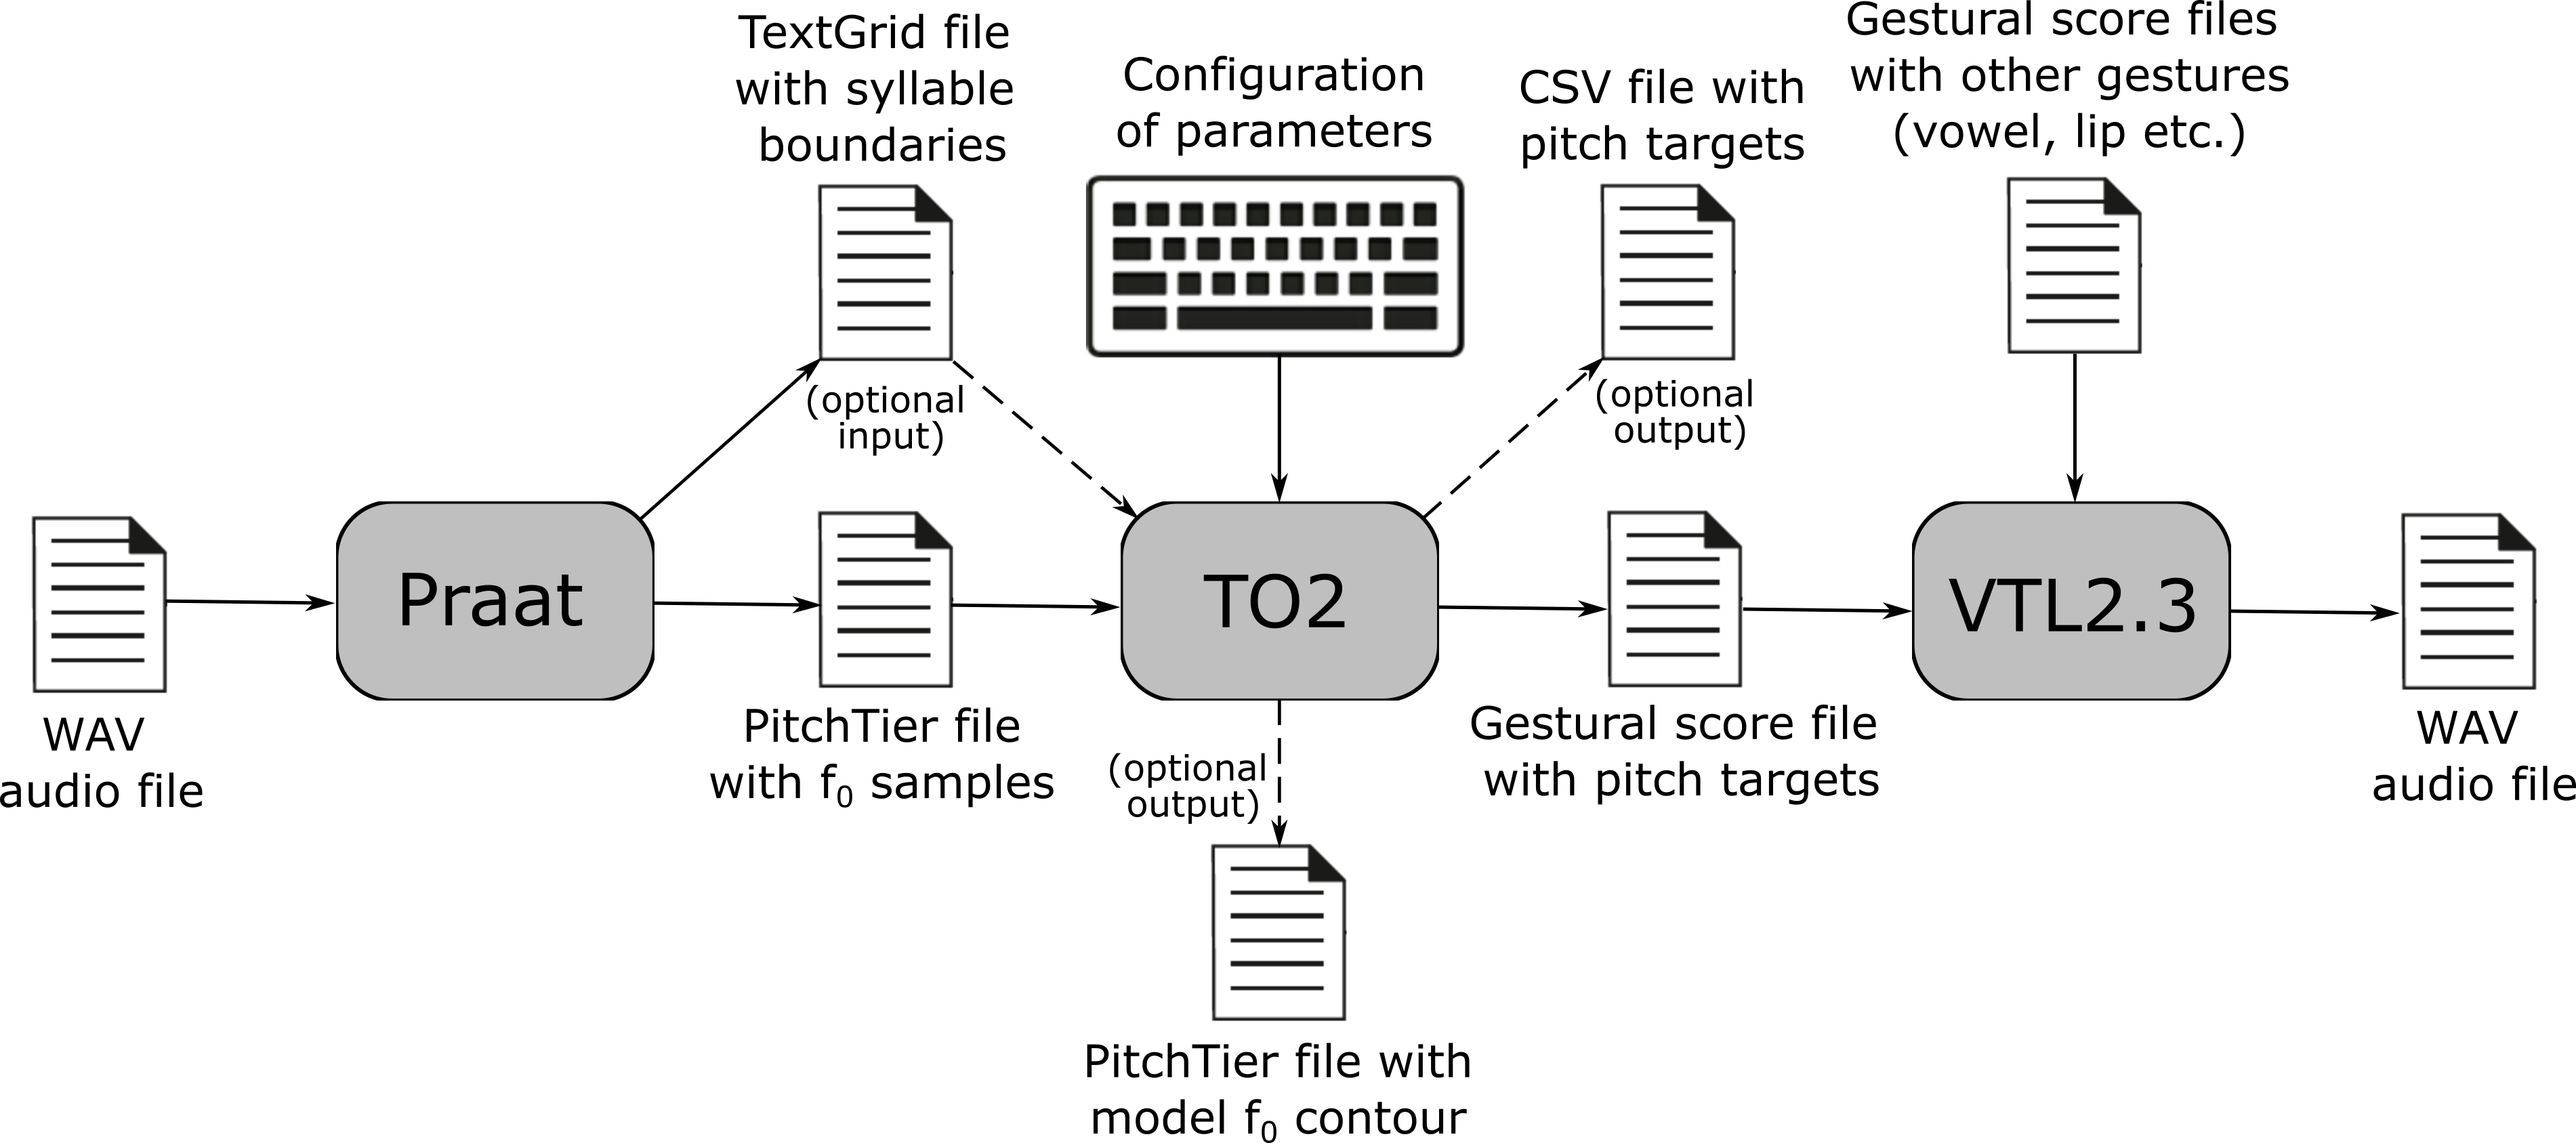
\includegraphics[width=0.9\textwidth]{images/flow.png}
\caption{
Articulatory speech synthesis pipeline}
\label{flow}
\end{figure}

In the following sections this workflow is shown step by step for the german word ``Ästhetik".

\section{Praat}

\begin{figure}[H]
\centering
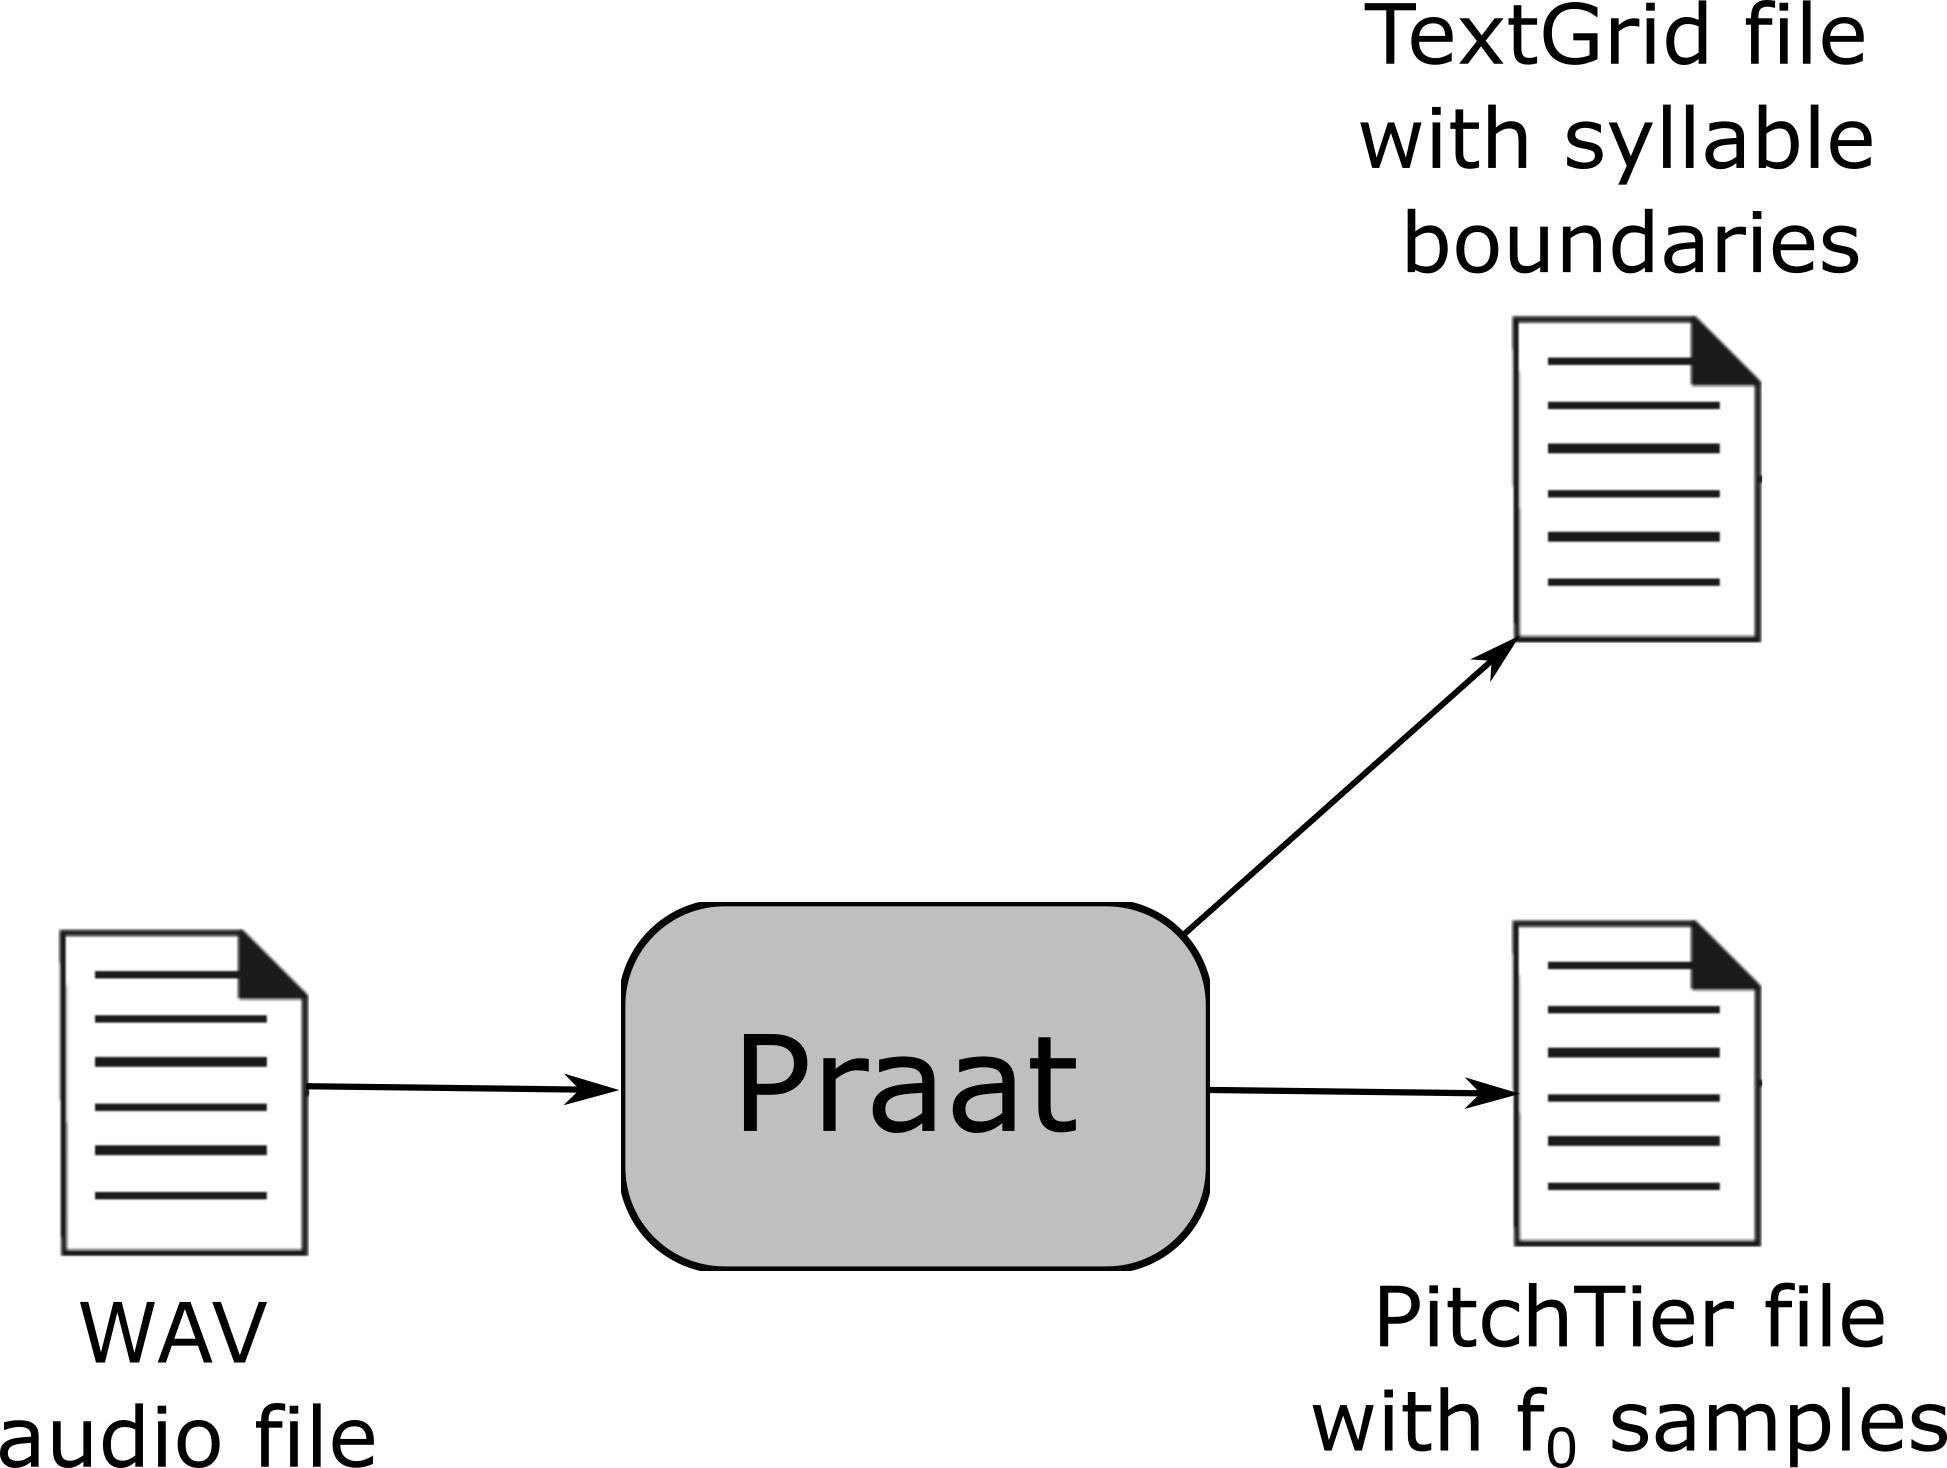
\includegraphics[width=0.4\textwidth]{images/3_11.png}
\caption{Input and outputs of Praat}
\label{3_11}
\end{figure}

Praat is used to obtain pitch frequencies and segment boundaries from a spoken utterance. Those information can be exported as a TextGrid file for the segment boundaries or as a PitchTier file for the pitch.\\
Therefore the utterance is imported into Praat and segmented. Segmentation takes place on syllable level and not phonetically. The pitch analysed is then extracted and those information exported. 

\begin{figure}[H]
\centering
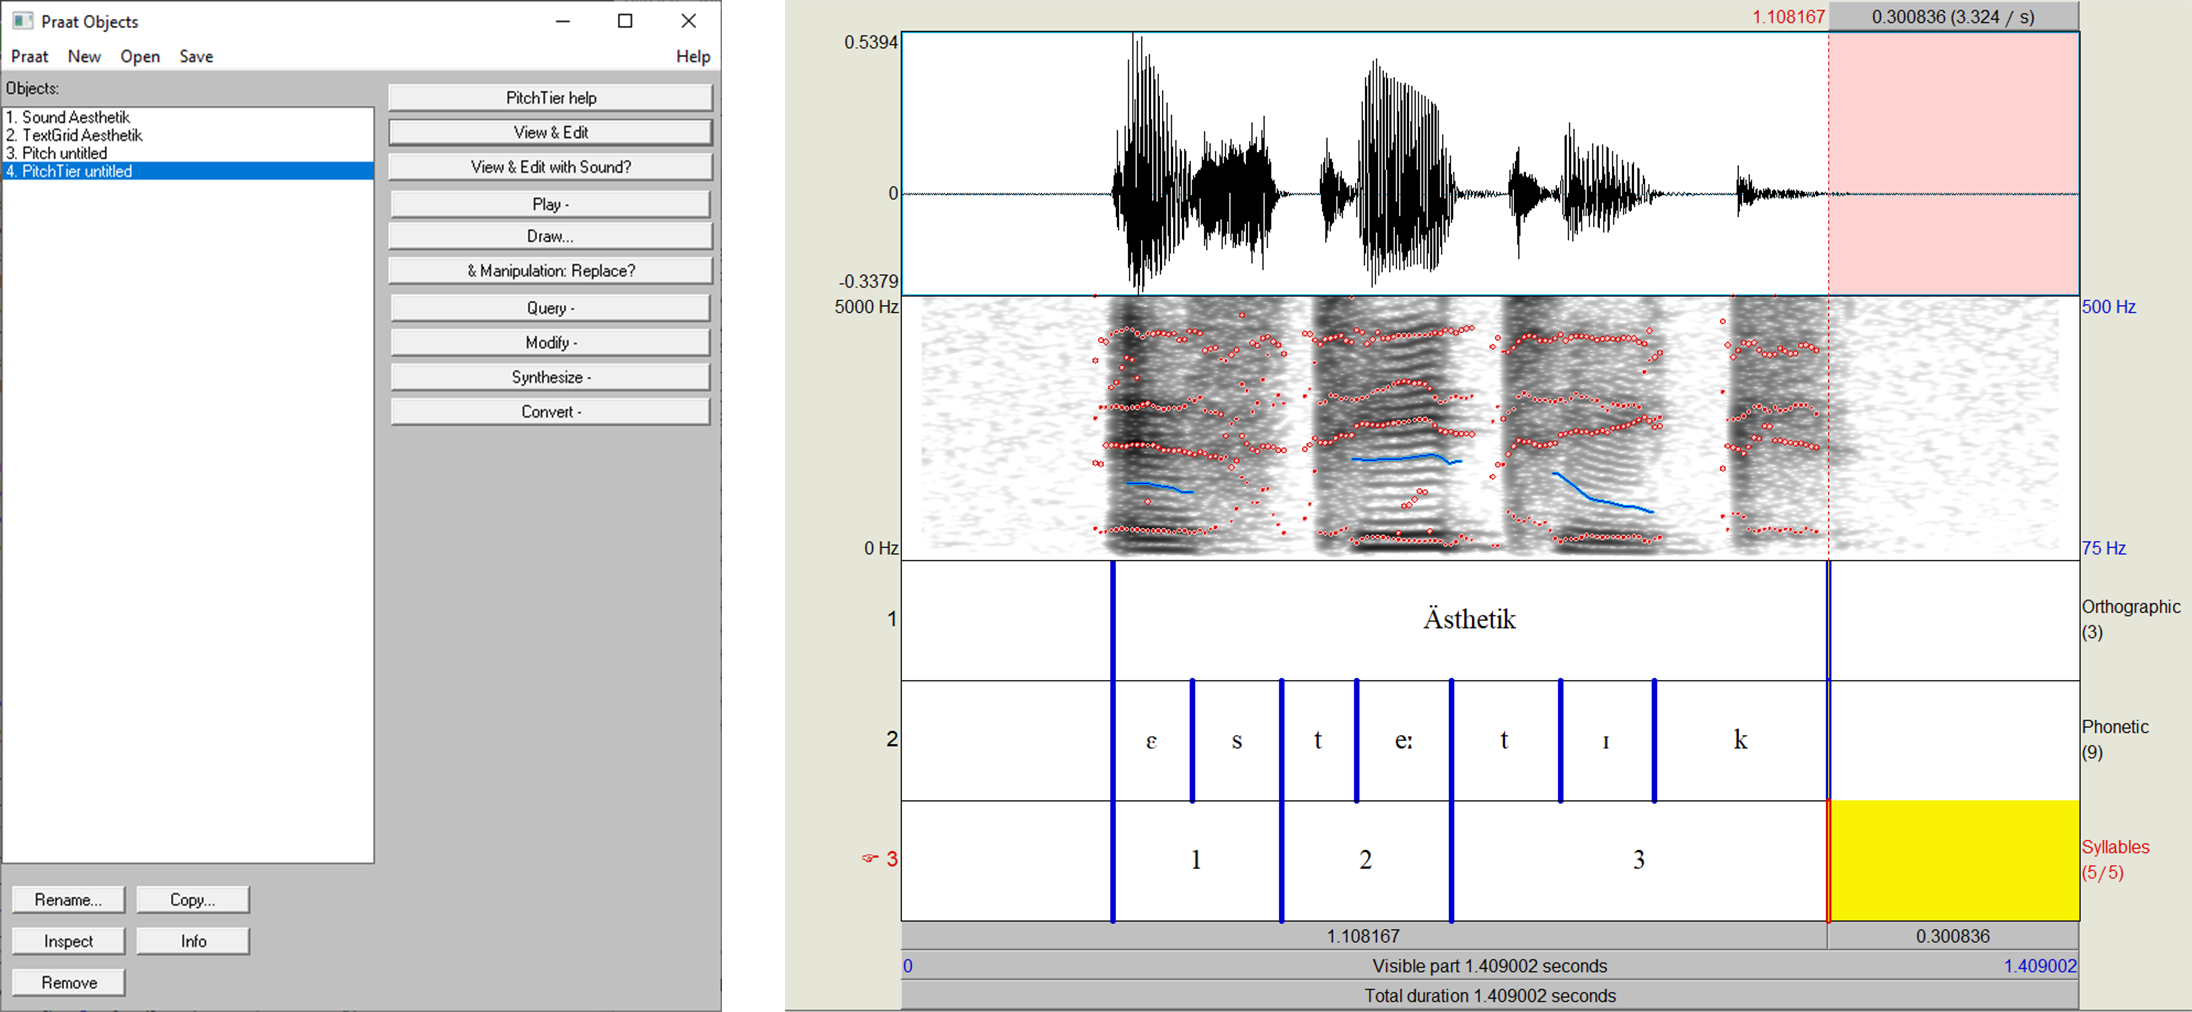
\includegraphics[width=0.9\textwidth]{images/3_12.png}
\caption{Praat GUIs: a) Objects Window, b) Editor Window}
\label{3_12}
\end{figure}

This procedure can be done with the following steps:

\begin{enumerate}
	\item In the Objects Window (see \autoref{3_12} a) ) import the sound file you want to analyse via ``Open" $\to$ ``Read from file..." or create a new record via ``New" $\to$ ``Record mono Sound...". A new Sound Object appears in the Objects Window list. 
	\item Select this Sound Object and use the function ``Annotate" $\to$ ``To TextGrid..." $\to$ $<$insert the tier names e.g. [Orthographic Phonetic Position]$>$ to obtain a new empty TextGrid which appears in the Objects Window list.
	\item Select both the Sound Object and the TextGrid Object and use the function View \& Edit to open both in the Editor Window. In this window you can segment and label the utterance in the tiers as you need it. Every change will be saved automatically in the TextGrid Object.
	\item In the Editor Window click on the menu ``Pitch" $\to$ ``Extract visible Pitch contour" to extract the automatically analysed pitch frequencies. A new Pitch Object appears in the Objects Window.
	\item Select the Pitch Object in the Object Window and use the function ``Convert" $\to$ ``Down to PitchTier". This creates a PitchTier Object. 
	\item To export the pitch frequencies in the PitchTier Object click on the menu `Save" $\to$ ``Save as PitchTier spreadsheet file..." and save the PitchTier file to your desired folder. 
	\item To export the target boundaries in the TextGrid Object click on the menu `Save" $\to$ ``Save as text file..." and save the TextGrid file to your desired folder. Be aware that the TO2 needs the TextGrid to be ecnoded in UTF-8 format. If you have special letters in the TextGrid file Praat is not able to convert this file to UTF-8. Please use another program to convert this file, e.g. Notepad++., before importing it in TO2.
\end{enumerate}

\section{TO2}

\begin{figure}[H]
\centering
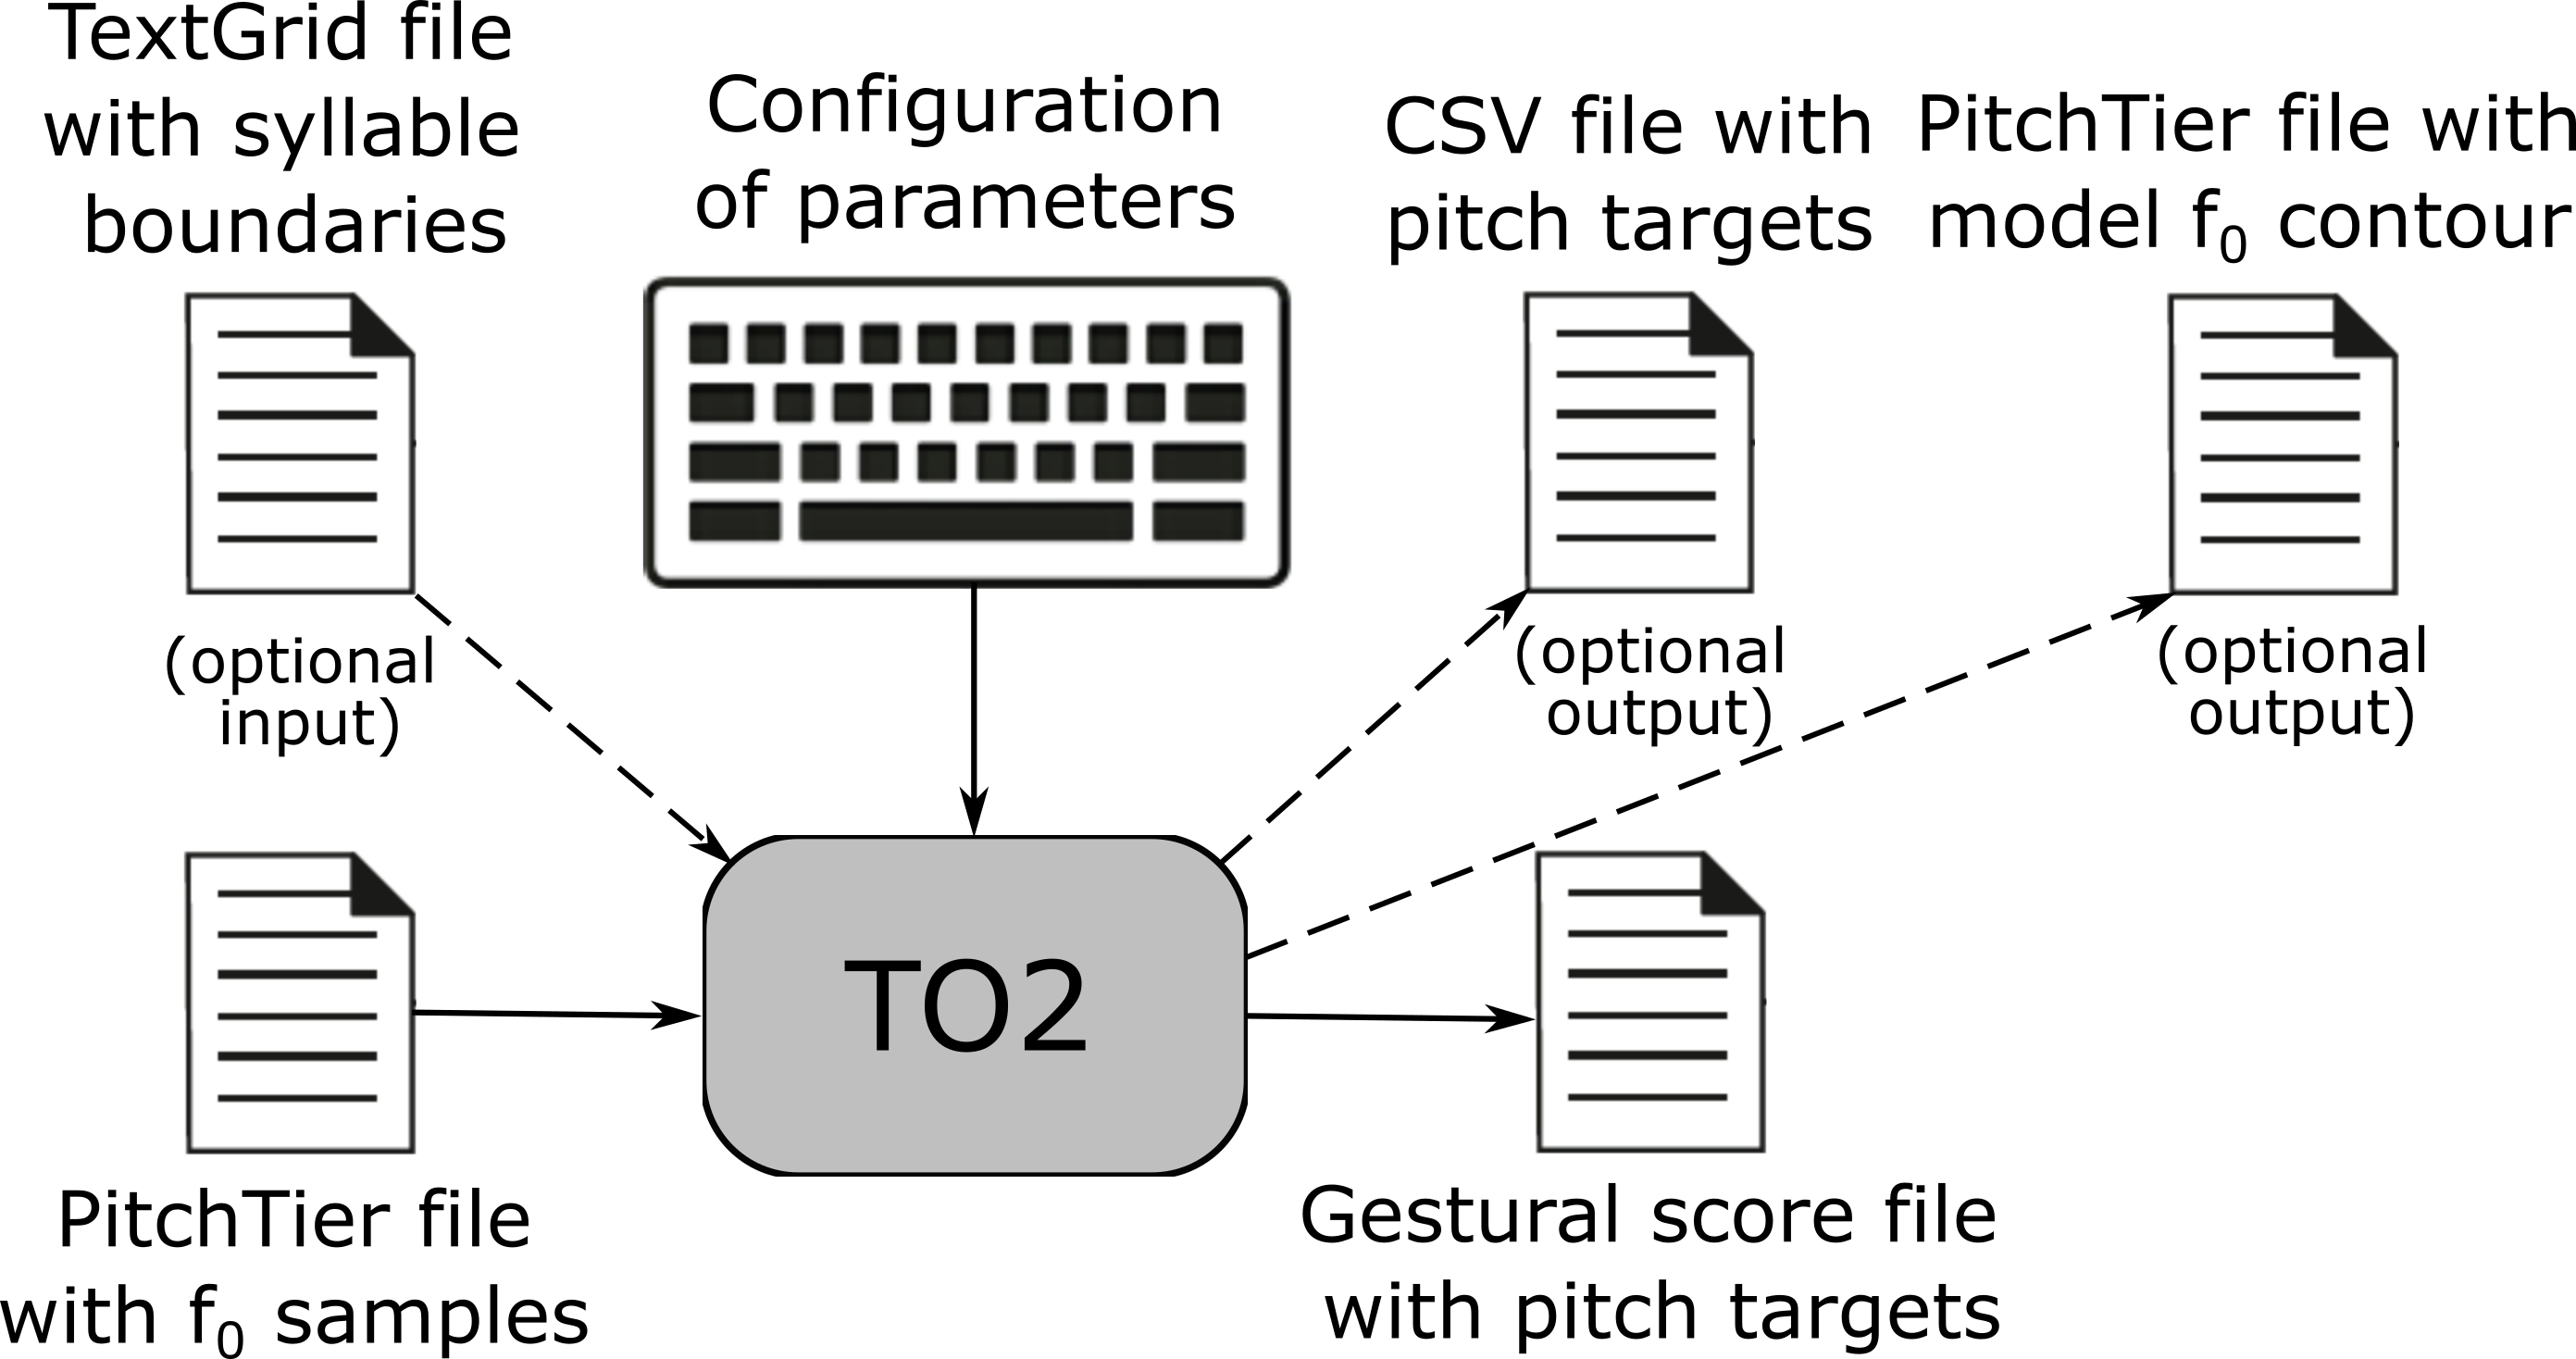
\includegraphics[width=0.4\textwidth]{images/3_21.png}
\caption{Input and outputs of TO2}
\label{3_21}
\end{figure}

The TO2 uses the PitchTier file and (not necessarily) the TextGrid file to perform a target optimization and obtain the pitch targets.

\begin{figure}[H]
\centering
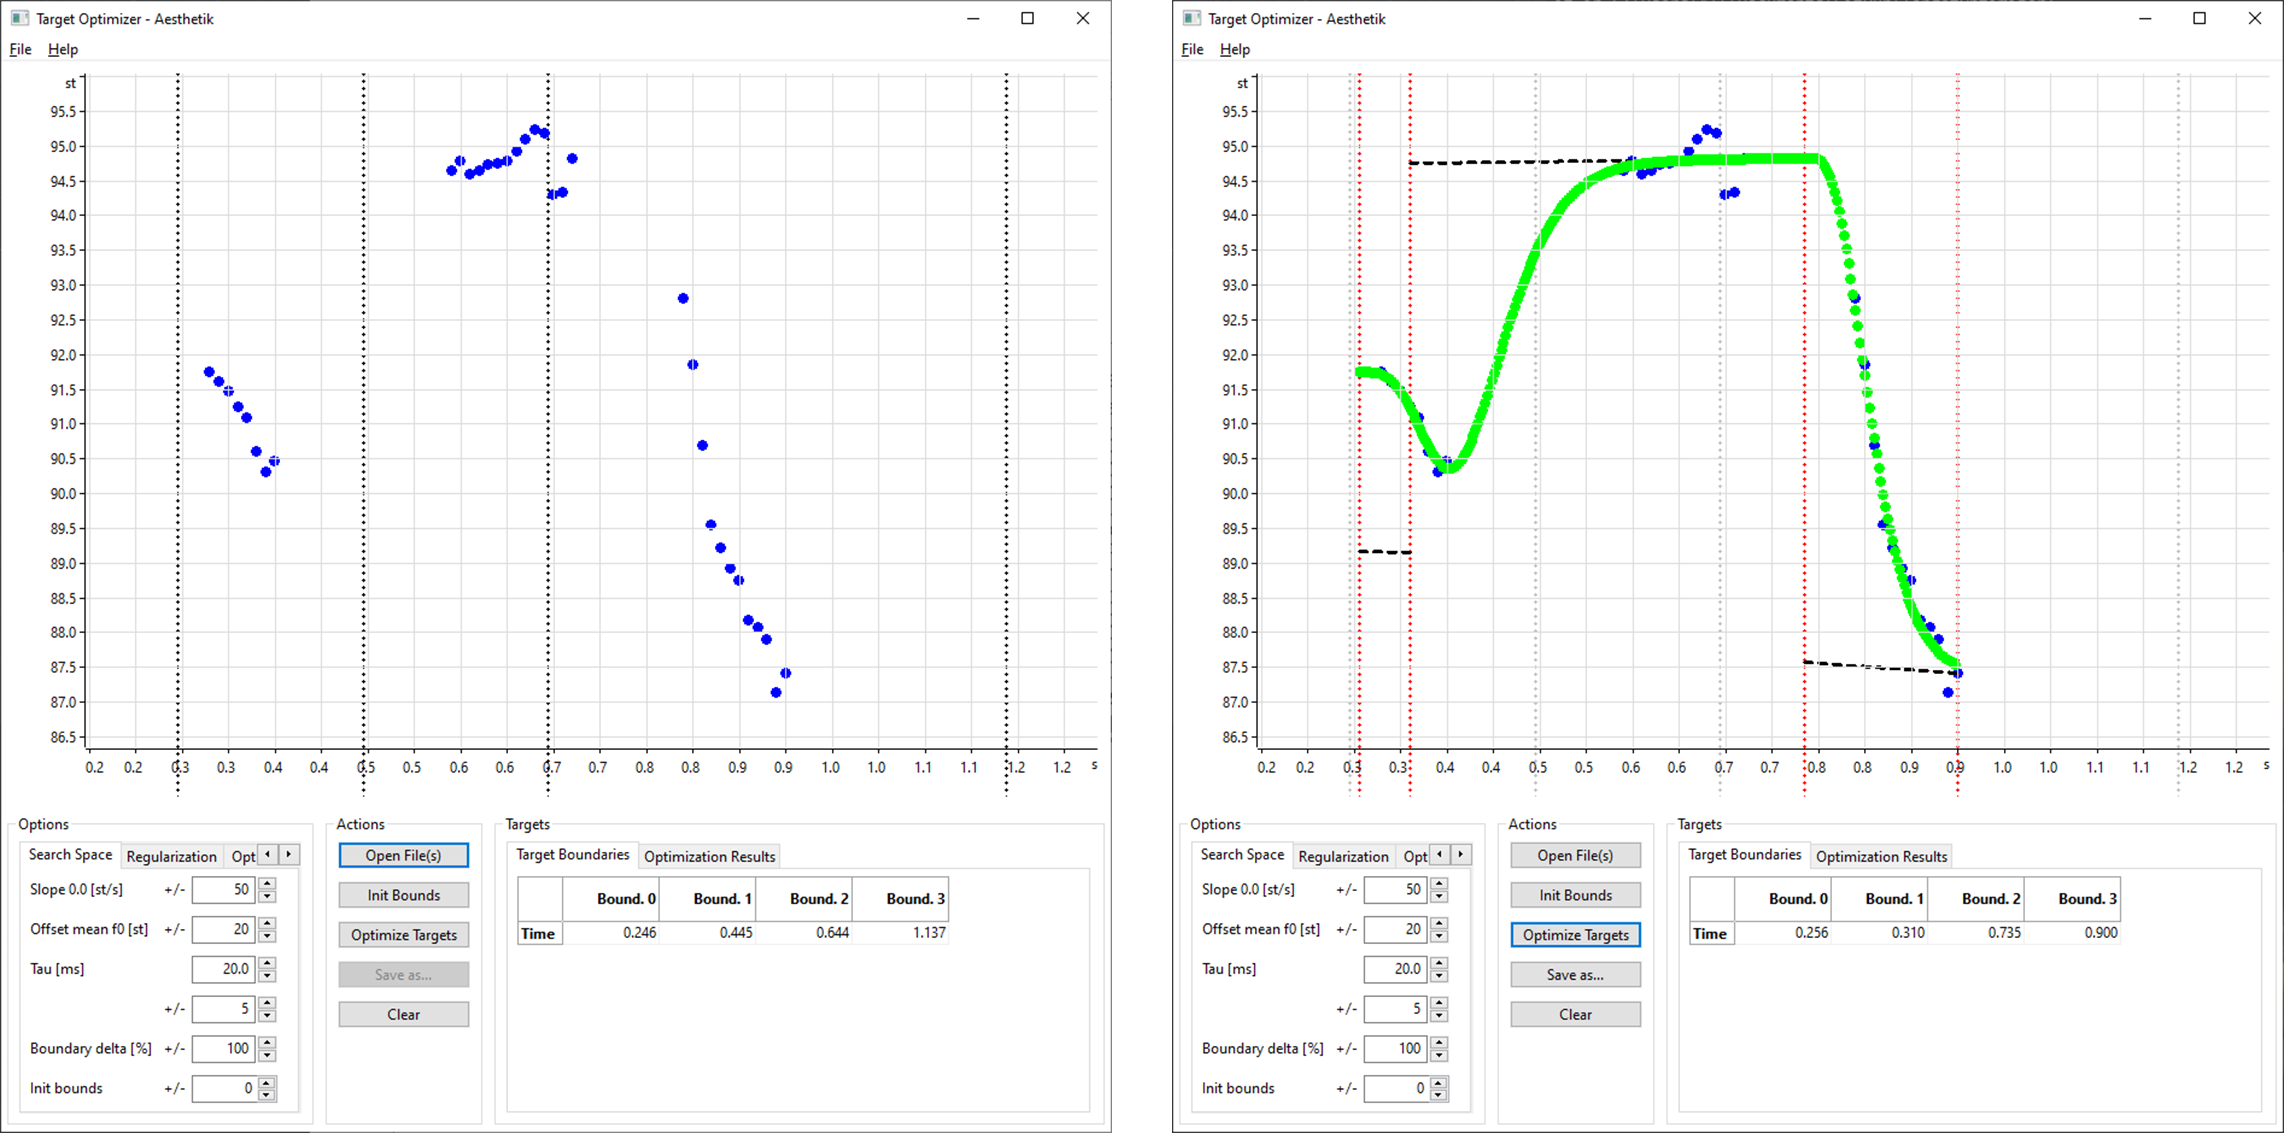
\includegraphics[width=0.9\textwidth]{images/3_22.png}
\caption{TO2 GUI: a) with imported PitchTier and TextGrid and b) with optimized pitch contour}
\label{3_22}
\end{figure}

Following steps are necessary to successfully estimate targets for an utterance:
\begin{enumerate}
	\item Open the pitch contour from the Praat PitchTier file.
	\item Input the corresponding boundaries. This can be performed by opening a Praat TextGrid file (UTF-8 encoded) or by using the equidistant boundary function of the TO2. To set equidistant boundaries type the amount of desired boundaries into ``Init bounds" option and click the ``Init Bounds" button. Afterwards the graph looks similar to Fig. \ref{3_22}a).
	\item Carefully think about the parameters you want to change (the default values are generally well suited).
	\item To perform the Target Approximation click the``Optimize" button. After the calculation the interpolated pitch contour is visible in the graph (see \autoref{3_22}b) ).
	\item Export the results as a *.ges file for VTL. 
\end{enumerate}

\section{VTL2.3}

\begin{figure}[H]
\centering
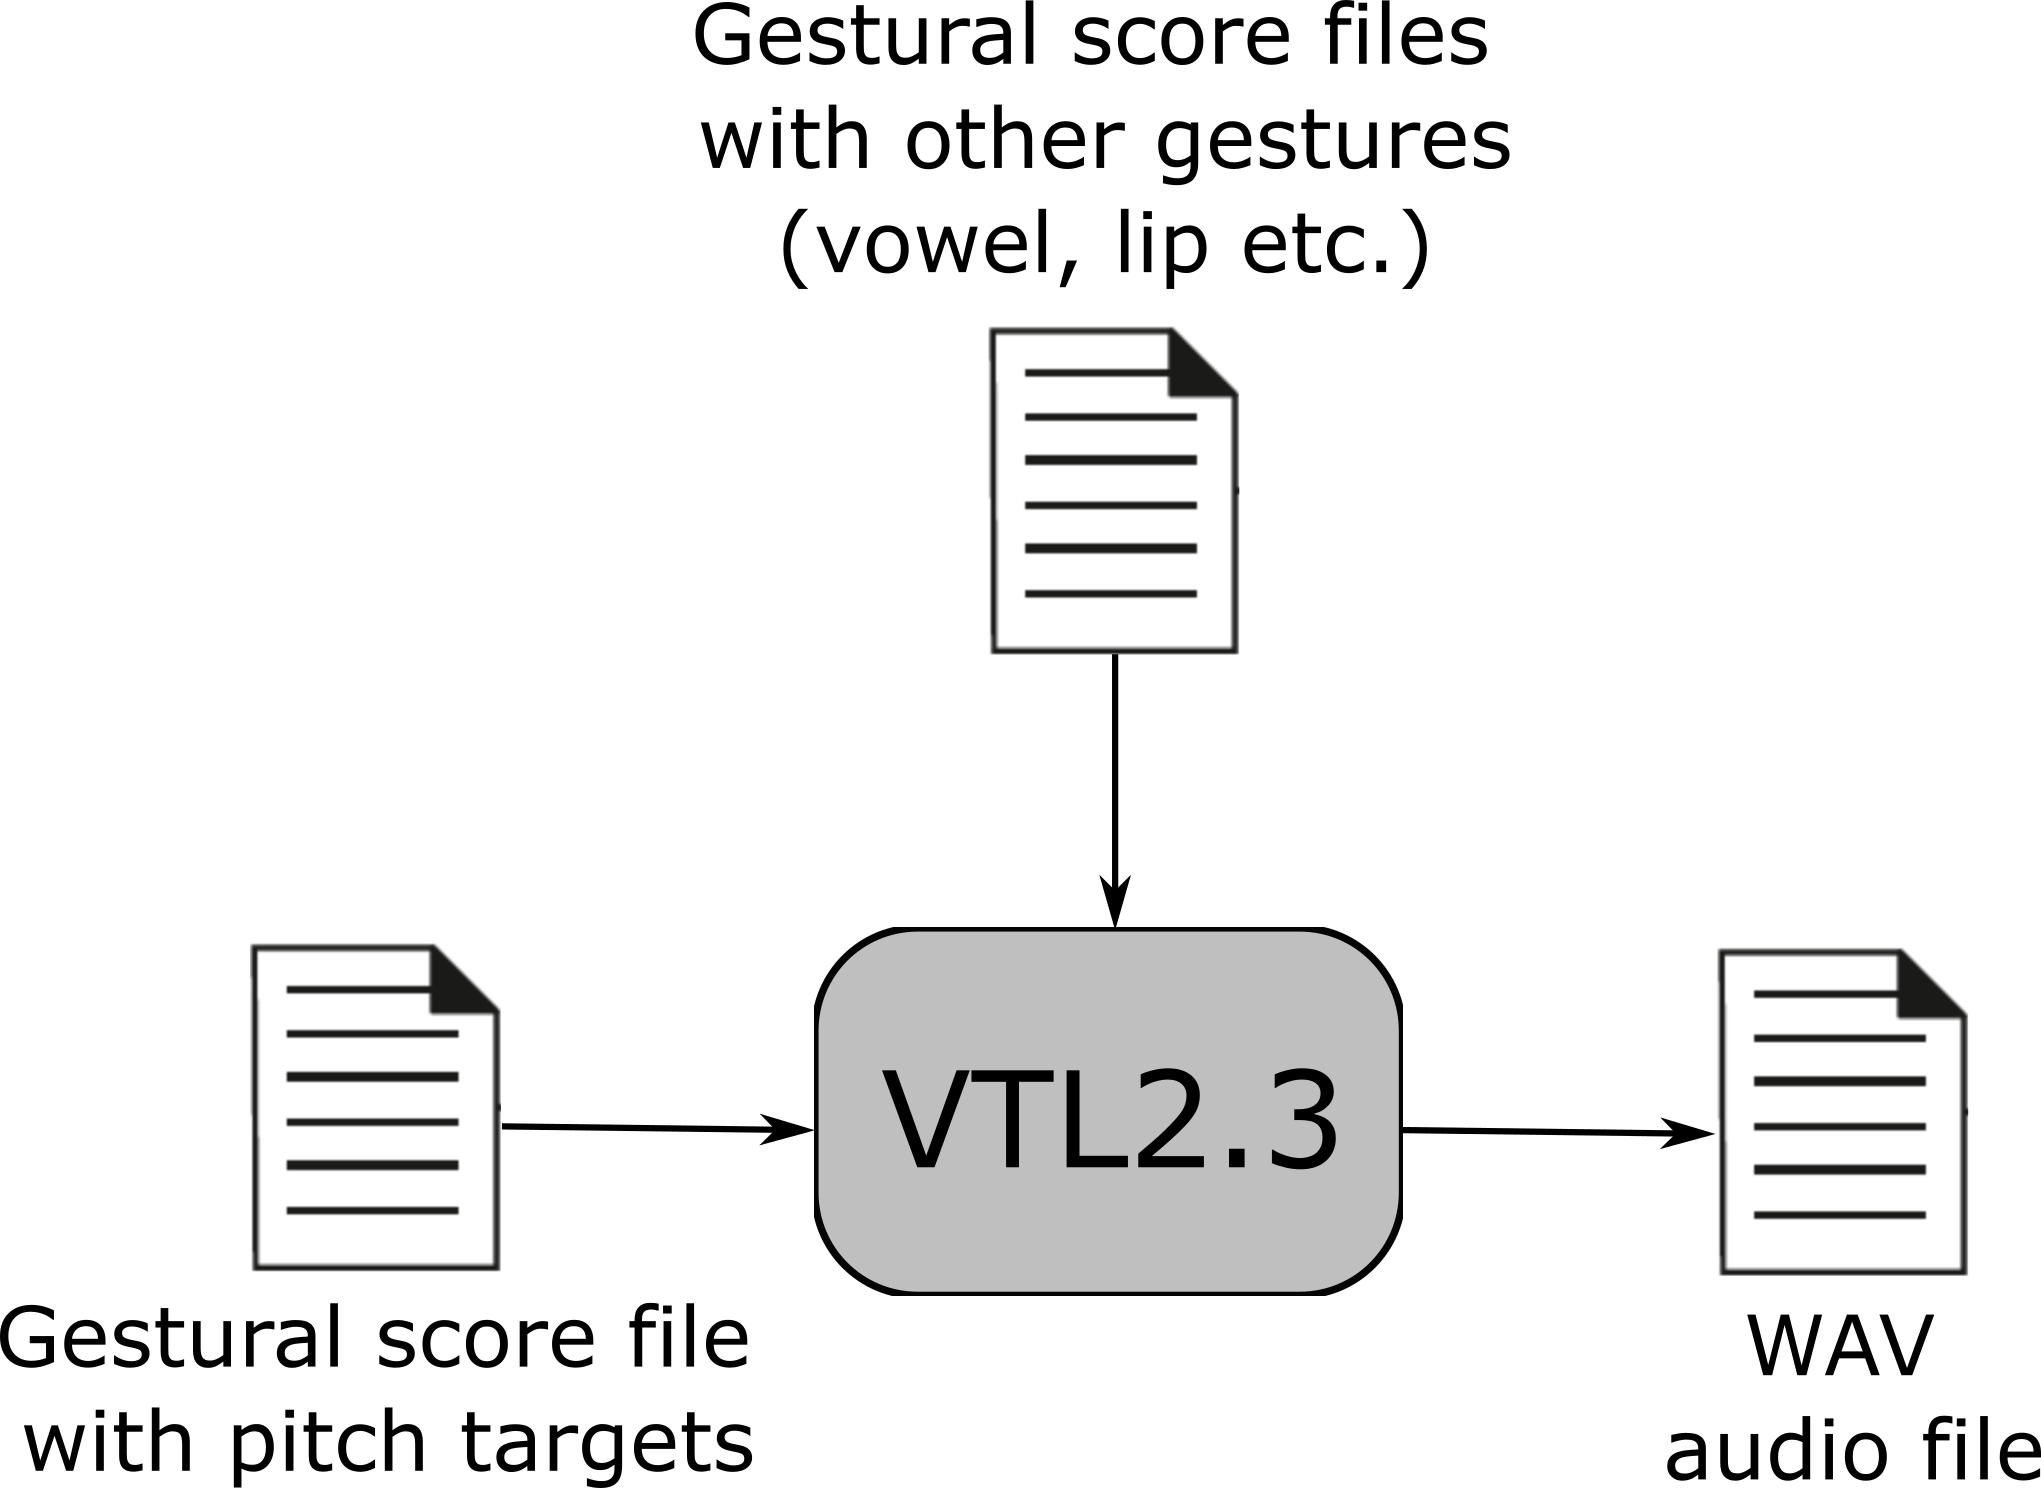
\includegraphics[width=0.4\textwidth]{images/3_31.png}
\caption{Input and outputs of VTL}
\label{3_31}
\end{figure}

The optimized pitch contour can now be used for articular speech synthesis in VTL. This can be done as follows:
\begin{enumerate}
	\item To import the pitch-contour information press ``File" $\to$ ``Load gestural score" and select the desired *.ges file.
	\item Click the ``Gestural score" in the toolbar to go to the gestural score page. In the gestural line ``F0 gestures" the information is now loaded and can be used for the synthesis.
\end{enumerate}